\documentclass[14pt, a4paper]{article}
\usepackage[utf8]{inputenc}
\usepackage[russian]{babel}
\usepackage{multirow}
\usepackage{graphicx}

\title{\textbf{Отчет о выполнении лабораторной работы 1.2.3}}
\author{Калашников Михаил, Б03-205}
\date{}

\begin{document}

\maketitle

Целью работы является измерение момента ряда тел и сравнение результатов с расчетами по теоретической формуле, проверка аддитивности моментов инерции.

В работе использовались трифилярный подвес, счетчик числа колебаний с секундомером, набор тел.

\begin{enumerate}

\item Перед началом измерений периодов колебаний я измерил параметры установки (табл. \ref{table1}).

\begin{table}[h]
\centering
\begin{tabular}{| c | c |}
\hline
Расстояние до точек подвеса & \\
подвижной платформы, $R$ & $115.5\pm 0.5\ mm$ \\
Расстояние до точек подвеса & \\
неподвижной платформы, $r$ & $30.2\pm 0.3\ mm$ \\
Масса ненагруженной & \\
платформы, $m_0$ & $1026\pm 0.5\ g$ \\
Радиус подвижной & \\
платформы, $R_0$ & $124.5\pm 1\ mm$ \\
Длина нити & \\
подвеса, $L$ & $2150\pm 10\ mm$ \\
Количество делений на & \\
подвижной платформе, $N_0$ & $25$ \\
\hline
\end{tabular}
\label{table1}
\caption{Параметры установки}
\end{table}

На основе этих данных может быть вычислена константа установки $k$ и ее погрешность $\sigma_k$ по формуле $\sigma_Y=\sqrt{\sum_{i=1}^N\left(\frac{\delta Y}{\delta X_i}\sigma_{X_i}\right)^2}$.

\[z_0=\sqrt{L^2-(R-r)^2}=2148\ mm\]
\[\sigma_{z_0}=\frac{1}{z_0}\sqrt{L^2\sigma_L^2+(R-r)^2(\sigma_R^2+\sigma_r^2)}=10\ mm\]

\[k=\frac{gRr}{4\pi^2z_0}=4.03\cdot10^{-4}\frac{m^2}{s^2}\]
\[\sigma_k=k\sqrt{\left(\frac{\sigma_R}{R}\right)^2+\left(\frac{\sigma_r}{r}\right)^2+\left(\frac{\sigma_{z_0}}{z_0}\right)^2}=0.05\cdot10^{-4}\frac{m^2}{s^2}\]

\item Измерим период колебаний ненагруженного подвеса. Результат занесем в таблицу \ref{table2}.

\begin{table}[h]
\centering
\begin{tabular}{| c | c | c |}
\hline
Измеренное время, $t,\ s$ & Кол-во колебаний, $N$ & Период колебаний $T_0,\ s$\\
\hline
92.7 & 21 & 4.41 \\
88.2 & 20 & 4.41 \\
88.0 & 20 & 4.40 \\
88.0 & 20 & 4.40 \\
88.2 & 20 & 4.41 \\
\hline
\end{tabular}
\label{table2}
\caption{Измерение момента инерции ненагруженного подвеса}
\end{table}

Период найдем как среднее значение, а погрешность определим как среднеквадратическое отклонение. Момент инерции вычисляется по формуле $I=kmT^2$.

\[T_0\pm \sigma_{T_0}=4.41\pm 0.002\ s\]
\[I_0\pm \sigma_{I_0}=8.04\pm 0.10\ g\cdot m^2\]

С другой стороны, момент инерции платформы может быть найден как момент инерции диска: $I_0=\frac{1}{2}mR_0^2=7.95\ g\cdot m^2$. Значение попадает в пределы погрешности.

\item Из набора тел выберем два тела: кольцо и диск с небольшим цилиндром в центре. Измерим период колебаний подвеса  и момент инерции системы с каждым из тел по отдельности и с двумя телами вместе.

\begin{table}[h]
\centering
\begin{tabular}{| c | c | c | c | c | c | c | c | c |}
\hline
\multicolumn{3}{| c |}{Диск ($m_1=584.2\pm0.1\ g$)} & \multicolumn{3}{| c |}{Кольцо ($m_2=737.5\pm0.1\ g$)} & \multicolumn{3}{| c |}{Диск + Кольцо} \\ 
\hline
$t,\ s$ & $N$ & $T_{01},\ s$ & $t,\ s$ & $N$ & $T_{02},\ s$ & $t,\ s$ & $N$ & $T_{012},\ s$ \\
\hline
86.7 & 22 & 3.94 & 85.0 & 20 & 4.25 & 79.7 & 20 & 3.99 \\
78.8 & 20 & 3.94 & 93.7 & 22 & 4.26 & 79.7 & 20 & 3.99 \\
86.6 & 22 & 3.94 & 85.3 & 20 & 4.27 & 79.6 & 20 & 3.98 \\
82.7 & 21 & 3.94 & 85.2 & 20 & 4.26 & 79.6 & 20 & 3.98 \\
79.0 & 20 & 3.95 & 85.3 & 20 & 4.27 & 103.4 & 26 & 3.98\\
\hline
\multicolumn{3}{| c |}{$T_{01}=3.94\pm 0.002\ s$} & \multicolumn{3}{| c |}{$T_{02}=4.26\pm 0.004\ s$} & \multicolumn{3}{| c |}{$T_{012}=3.98\pm 0.002\ s$} \\
\multicolumn{3}{| c |}{$I_{01}=10.10\pm 0.12\ g\cdot m^2$} & \multicolumn{3}{| c |}{$I_{02}=12.93\pm 0.15\ g\cdot m^2$} & \multicolumn{3}{| c |}{$I_{012}=15.04\pm 0.18\ g\cdot m^2$} \\
\hline
\end{tabular}
\label{table3}
\caption{Измерение момента инерции нагруженного подвеса}
\end{table}

Теперь можно вычислить моменты инерции тел и убедиться, что аддитивность выполнена в пределах погрешности:

\[I_1=I_{01}-I_0=2.06\pm 0.22\ g\cdot m^2\]
\[I_2=I_{02}-I_0=4.89\pm 0.25\ g\cdot m^2\]
\[I_{12}=I_1+I_2=6.95\pm 0.37\ g\cdot m^2\]
\[I_{12}=I_{012}-I_0=7.00\pm 0.28\ g\cdot m^2\]

Произведем расчет моментов инерции обоих тел теоретически. Занесем геометрические размеры тел в таблицу.

\begin{table}[h]
\centering
\begin{tabular}{| c | c |}
\hline
\multicolumn{2}{| c |}{Диск} \\
\hline
Радиус диска, $R_d$ & $85.2\ mm$ \\
Толщина диска, $W_d$ & $3.25\ mm$ \\
Радиус центрального цилиндра, $r$ & $6\ mm$ \\
Высота центрального цилиндра, $h$ & $27\ mm$ \\
\hline
\multicolumn{2}{| c |}{Кольцо} \\
\hline
Внешний радиус кольца, $R_{ex}$ & $83.2\ mm$ \\
Внутренний радиус кольца, $R_{in}$ & $78.2\ mm$ \\
\hline
\end{tabular}
\label{table4}
\caption{Геометрические размеры исследуемых тел}
\end{table}

Момент инерции диска можно найти как сумму моментов инерций двух сплошных цилиндров:

\[m_{1a}=\frac{V_{1a}}{V_{1a}+V_{1b}}m_1=\frac{R_d^2W_d}{R_d^2W_d+r^2h^2}m_1,\ m_{2a}=\frac{V_{2a}}{V_{1a}+V_{1b}}m_1=\frac{r^2h}{R_d^2W_d+r^2h^2}m_1\]
\[I_{1th}=\frac{1}{2}m_{1a}R_d^2+\frac{1}{2}m_{1b}r^2=\frac{R_d^4W_d+r^4h}{R_d^2W_d+r^2h}\frac{m_1}{2}=2.04\ g\cdot m^2\]

Момент инерции кольца вычисляется по формуле:

\[I_{2th}=m_2\frac{R_{ex}^2+R_{in}^2}{2}=4.81\ g\cdot m^2\]

С учетом погрешности, моменты инерции, полученные в теории и на практике, совпадают.

\item Поместим на платформу диск, разрезанный по диаметру. Будем измерять период колебаний, постепенно раздвигая половинки. На основе периода и массы половинок ($m_3=1527.1\ g$) рассчитаем момент инерции системы, в зависимости от h. Результаты занесем в таблицу.

\begin{table}[h]
\centering
\begin{tabular}{| c | c | c | c | c |}
\hline
Расстояние до & Измеренное & Кол-во & Период, & Момент \\
центра, $h, cm$ & время, $t,\ s$ &колебаний, $N$ & $T_{03}, s$ & инерции $I_{03},\ g\cdot m^2$ \\
\hline
%\multirow{2}{*}{0.00} & 64.7 & 21 & \multirow{2}{*}{3.08} & \multirow{2}{*}{9.76} \\
%& 61.4 & 20 & & \\
%\hline
%\multirow{2}{*}{24.90} & 64.3 & 20 & \multirow{2}{*}{3.14} & \multirow{2}{*}{10.14} \\
%& 64.4 & 20  & & \\
%\hline
\multirow{2}{*}{44.82} & 53.0 & 15 & \multirow{2}{*}{3.53} & \multirow{2}{*}{12.82} \\
\hline
& 70.5 & 20 & & \\
\hline
\multirow{2}{*}{59.76} & 57.5 & 15 & \multirow{2}{*}{3.83} & \multirow{2}{*}{15.09} \\
& 57.5 & 15 & & \\
\hline
\multirow{2}{*}{69.72} & 61.2 & 15 & \multirow{2}{*}{4.08} & \multirow{2}{*}{17.13} \\
& 61.2 & 15 & & \\
\hline
\multirow{2}{*}{79.68} & 65.2 & 15 & \multirow{2}{*}{4.34} & \multirow{2}{*}{19.38} \\
& 65.1 & 15 & & \\
\hline
\multirow{2}{*}{89.64} & 69.6 & 15 & \multirow{2}{*}{4.64} & \multirow{2}{*}{22.15} \\
& 83.5 & 18 & & \\
\hline
\end{tabular}
\label{table5}
\caption{Измерение момента инерции разрезанного диска}
\end{table}

Построим график зависимости $I_{03}(h^2)$: проведем через полученные точки прямую с помощью МНК. Момент инерции диска может быть выражен следующим образом: 
\[I_3=I_{03}(0)-I_{0}=1.59\ g\cdot m^2.\]

С другой стороны ($R_3=45.51\ mm$):
\[I_{3th}=\frac{1}{2}m_3R_3^2=1.58\ g\cdot m^2.\]

Точность составляет 0.6\%.



\begin{figure}[h]
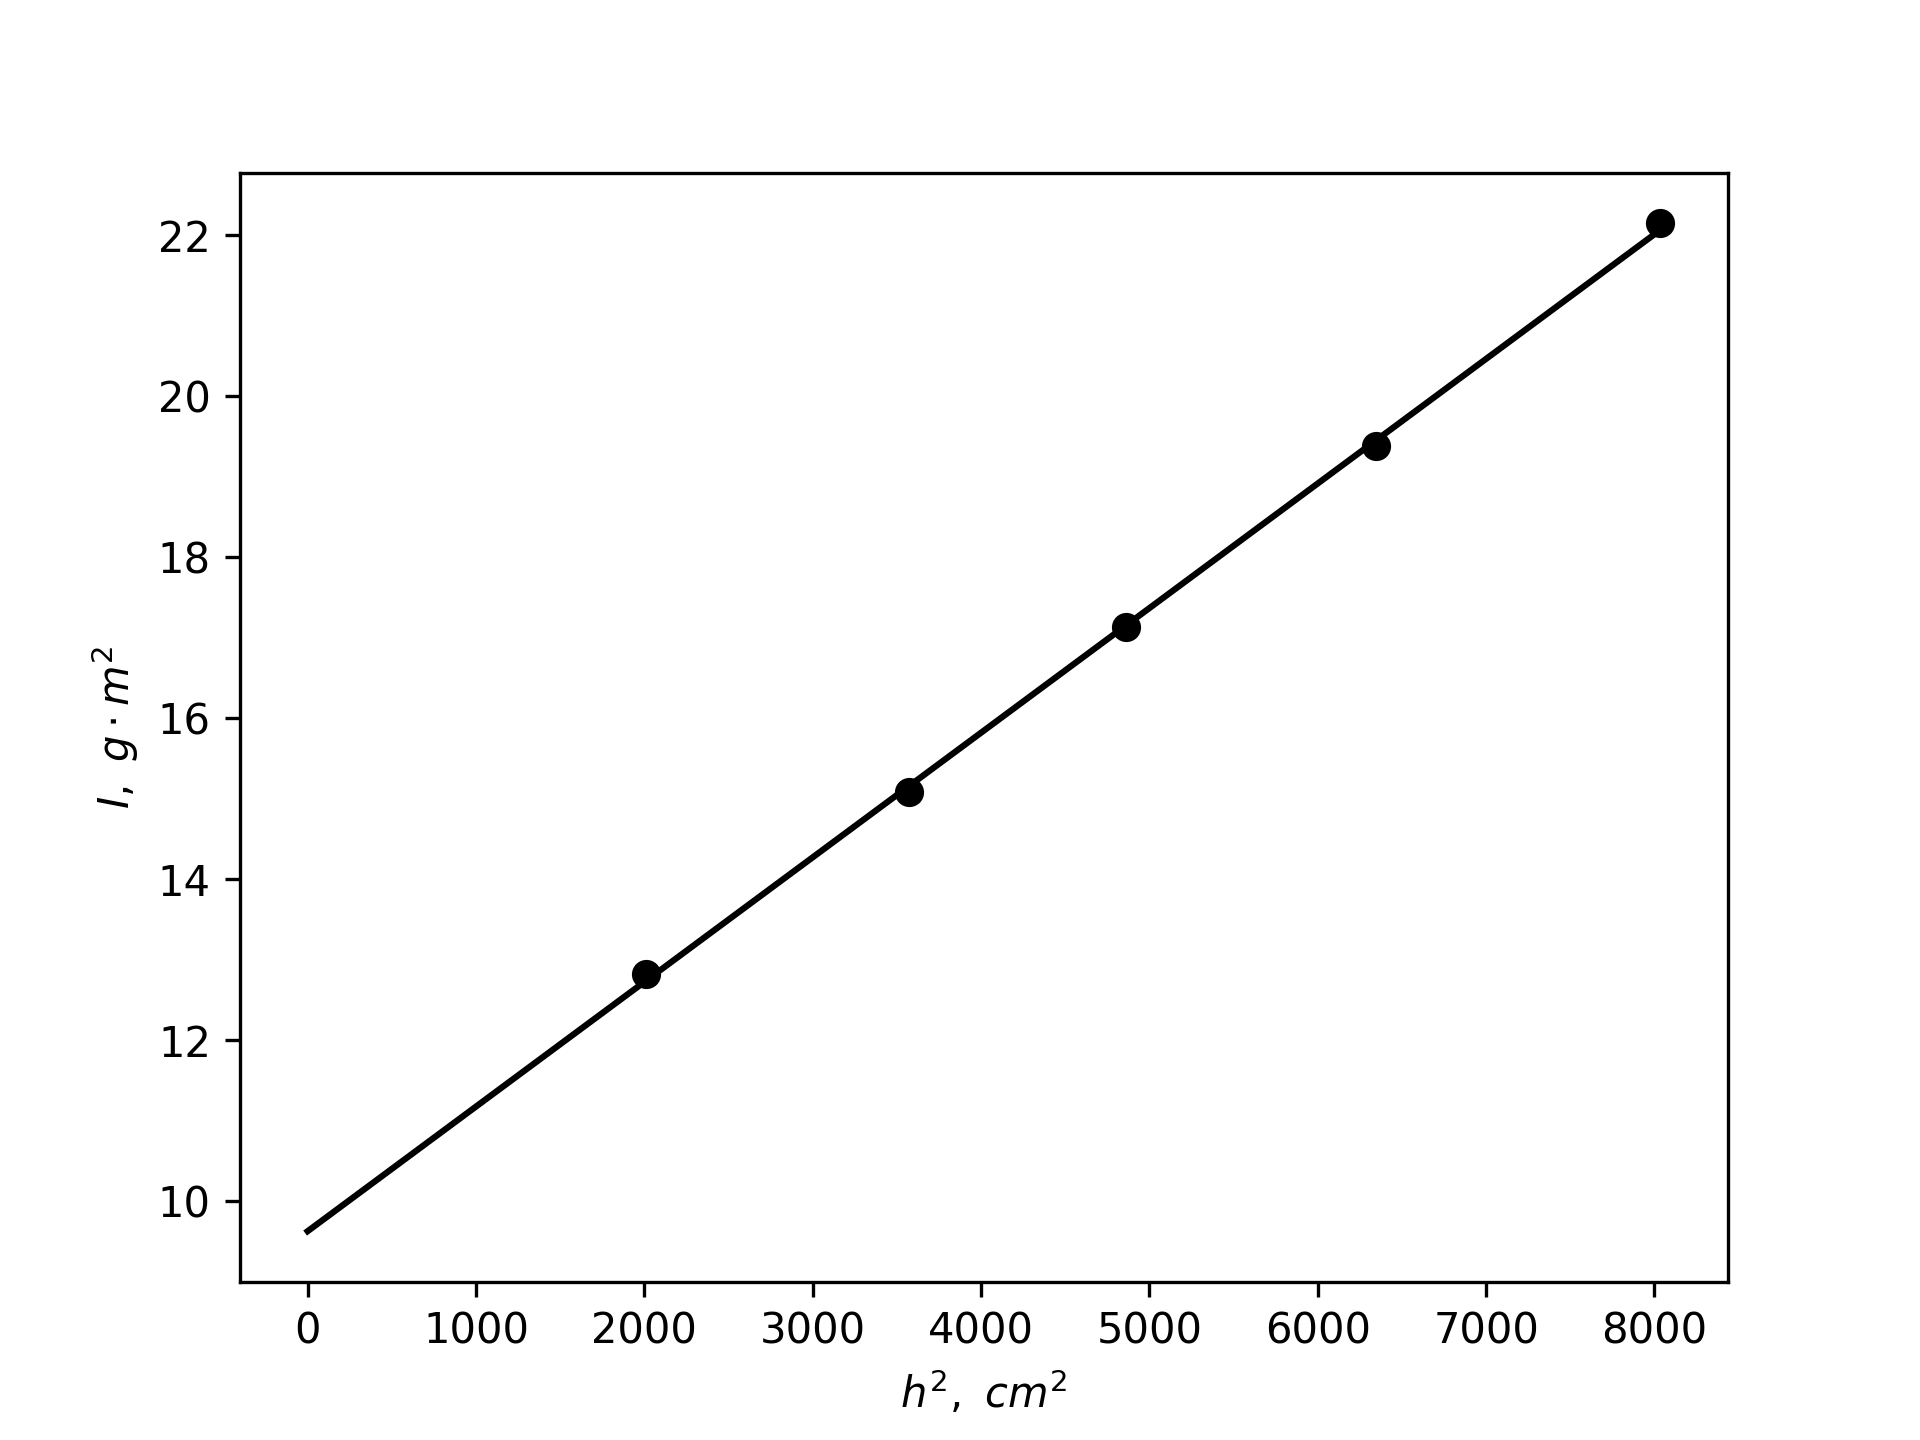
\includegraphics[width=\linewidth]{laba4_1.png}
\caption{График зависимости $I(h^2)$}
\label{image1}
\end{figure}

\end{enumerate}

\end{document}